\documentclass[twoside,11pt,preprint]{article}

\usepackage{dmlr2e}
\usepackage{booktabs}
\usepackage{url}

% Generated by paper/scripts/build_paper_assets.py. Do not edit by hand.
\newcommand{\MainGraphClusters}{20}
\newcommand{\InteractionP}{0.488}
\newcommand{\InteractionEffectRangePP}{30}
\newcommand{\StudyModels}{5}
\newcommand{\StudyMainPairs}{100}
\newcommand{\StudyMainBaseCorrect}{73}
\newcommand{\StudyMainDistCorrect}{45}
\newcommand{\StudyMainDeltaPP}{-28.0}
\newcommand{\StudyMainCILowPP}{-41.0}
\newcommand{\StudyMainCIHighPP}{-15.0}
\newcommand{\StudyMainSignFlipP}{0.0011}
\newcommand{\StudyBaselineOnly}{34}
\newcommand{\StudyDistractorOnly}{6}
\newcommand{\StudyMainPositiveGraphs}{2}
\newcommand{\StudyMainZeroGraphs}{4}
\newcommand{\StudyMainNegativeGraphs}{14}
\newcommand{\StudyASPP}{+26.0}
\newcommand{\StudyASPCILowPP}{+12.7}
\newcommand{\StudyASPCIHighPP}{+38.7}
\newcommand{\StudyASPSignFlipP}{0.0039}
\newcommand{\StudyASPPositiveGraphs}{11}
\newcommand{\StudyASPZeroGraphs}{2}
\newcommand{\StudyASPNegativeGraphs}{2}
\newcommand{\ASPRangeLowPP}{+20.0}
\newcommand{\ASPRangeHighPP}{+46.7}
\newcommand{\MiniMaxASPP}{+46.7}
\newcommand{\MiniMaxASPLowPP}{+23.3}
\newcommand{\MiniMaxASPHighPP}{+70.0}
\newcommand{\MiniMaxASPHolmP}{0.0342}
\newcommand{\DeepSeekBaseCorrect}{20}
\newcommand{\DeepSeekBaseTrials}{20}
\newcommand{\DeepSeekDistCorrect}{14}
\newcommand{\DeepSeekDistTrials}{20}
\newcommand{\DeepSeekDeltaPP}{-30.0}
\newcommand{\DeepSeekDeltaLowPP}{-50.0}
\newcommand{\DeepSeekDeltaHighPP}{-10.0}
\newcommand{\DeepSeekMcNemarP}{0.0312}
\newcommand{\DeepSeekHolmP}{0.1250}
\newcommand{\KimiBaseCorrect}{13}
\newcommand{\KimiBaseTrials}{20}
\newcommand{\KimiDistCorrect}{7}
\newcommand{\KimiDistTrials}{20}
\newcommand{\KimiDeltaPP}{-30.0}
\newcommand{\KimiDeltaLowPP}{-55.0}
\newcommand{\KimiDeltaHighPP}{-5.0}
\newcommand{\KimiMcNemarP}{0.0703}
\newcommand{\KimiHolmP}{0.2109}
\newcommand{\GLMBaseCorrect}{7}
\newcommand{\GLMBaseTrials}{20}
\newcommand{\GLMDistCorrect}{5}
\newcommand{\GLMDistTrials}{20}
\newcommand{\GLMDeltaPP}{-10.0}
\newcommand{\GLMDeltaLowPP}{-35.0}
\newcommand{\GLMDeltaHighPP}{+15.0}
\newcommand{\GLMMcNemarP}{0.6875}
\newcommand{\GLMHolmP}{0.6875}
\newcommand{\MiniMaxBaseCorrect}{16}
\newcommand{\MiniMaxBaseTrials}{20}
\newcommand{\MiniMaxDistCorrect}{8}
\newcommand{\MiniMaxDistTrials}{20}
\newcommand{\MiniMaxDeltaPP}{-40.0}
\newcommand{\MiniMaxDeltaLowPP}{-65.0}
\newcommand{\MiniMaxDeltaHighPP}{-15.0}
\newcommand{\MiniMaxMcNemarP}{0.0215}
\newcommand{\MiniMaxHolmP}{0.1074}
\newcommand{\QwenBaseCorrect}{17}
\newcommand{\QwenBaseTrials}{20}
\newcommand{\QwenDistCorrect}{11}
\newcommand{\QwenDistTrials}{20}
\newcommand{\QwenDeltaPP}{-30.0}
\newcommand{\QwenDeltaLowPP}{-60.0}
\newcommand{\QwenDeltaHighPP}{-5.0}
\newcommand{\QwenMcNemarP}{0.1094}
\newcommand{\QwenHolmP}{0.2188}


\ShortHeadings{Affordance-Controlled Tool-Use Evaluation}{Authors withheld}
\firstpageno{1}

\begin{document}

\title{Affordance-Controlled Evaluation of Multi-Step Tool Use:\\
Connected-Compatible Distractors and Model-Specific Degradation}

\author{Author information withheld in working draft}

\maketitle

\begin{abstract}
Multi-step function-calling evaluations often report final success for a task
distribution in which many properties vary at once: the number of exposed tools,
their structural relation to the goal, and whether an irrelevant branch is
actually executable. Building on the hidden dependency-graph mechanism of
FuncBenchGen, we study a narrower measurement question. When the required
dependency subgraph, target truth, inputs, prompt, and core tool order are held
fixed, does adding connected, type-compatible, executable distractors degrade
multi-step tool use? We evaluate five API-served models on \MainGraphClusters{}
independently generated depth-three graphs. Five connected-compatible
distractors are associated with a decline from \DeepSeekBaseCorrect/\DeepSeekBaseTrials{}
to \DeepSeekDistCorrect/\DeepSeekDistTrials{} for DeepSeek Flash,
\KimiBaseCorrect/\KimiBaseTrials{} to \KimiDistCorrect/\KimiDistTrials{} for
Kimi K3.1 Pro, \GLMBaseCorrect/\GLMBaseTrials{} to
\GLMDistCorrect/\GLMDistTrials{} for GLM-5.3-Flashx,
\MiniMaxBaseCorrect/\MiniMaxBaseTrials{} to
\MiniMaxDistCorrect/\MiniMaxDistTrials{} for MiniMax-M3.1-Flash, and
\QwenBaseCorrect/\QwenBaseTrials{} to \QwenDistCorrect/\QwenDistTrials{} for
Qwen3.8-Max. These are descriptive declines of approximately 30, 30, 10, 40, and 30
percentage points, respectively. The model ordering does not reverse, and a
graph-cluster permutation test does not establish model-interaction
heterogeneity (p=\InteractionP). On 15 shared control graphs, five
disconnected tools and five connected-incompatible tools do not reproduce the
degradation observed for five connected-compatible tools, although the control
sample remains bounded. Structured traces show lower function-selection precision under
distractors, while errors include wrong arguments, premature dependency use,
irrelevant calls, and premature final answers. A 0/2/5 study on 15 graphs is more
consistent with model-specific plateaus or threshold-like behavior than with a
common linear dose response. Neither a state reminder nor prerequisite hiding
improves success. The study is a controlled diagnostic evaluation, not a
comprehensive model ranking, a claim of contamination immunity, or evidence of a
successful repair.
\end{abstract}

\begin{keywords}
multi-step function calling, tool-use evaluation, procedural benchmark
generation, counterfactual data design, distractor affordance, structured tool
traces
\end{keywords}

\section{Introduction}

Large language models increasingly call external functions over multiple turns.
A successful trajectory must do more than emit syntactically valid calls. It
must choose a goal-relevant function, supply values produced by earlier calls,
respect dependencies, avoid irrelevant branches, and terminate after the target
is reached. Benchmarks for API use have therefore examined API selection,
argument construction, planning, and multi-tool execution at different levels
of realism and scale \citep{li2023apibank,qin2023toolllm,patil2023gorilla,
shen2024taskbench}. Yet final success still conflates several properties of a
task's data design.

Procedurally generated benchmarks reduce exact instance reuse and make some
complexity variables controllable
\citep{srivastava2025beyondbench,li2025c2leva,chen2025dycodeeval}. They do not
by themselves establish which change made a task harder. In particular, adding
candidate tools changes the number of options, the number of connected graph
nodes, the availability of their input types, and whether an incorrect branch can
be executed. A comparison between zero and many distractors therefore mixes
candidate-set size with \emph{affordance}: the extent to which the environment
affords plausible but goal-irrelevant actions.

FuncBenchGen already turns tool use into traversal of a hidden
function-dependency DAG and already includes type-compatible distractor
functions \citep{maekawa2025funcbenchgen}. Our contribution is not the invention
of that generator. We ask whether a stricter counterfactual design around the
same required subgraph can isolate the role of executable connected distractors,
and whether trace-level outcomes reveal how the resulting failures are
distributed. We also test two intuitive state-support interventions rather than
assuming that a better prompt or a smaller candidate set must repair the
problem.

This evaluation is deliberately narrow. It uses one function-dependency task
family, fixed dependency depth three, five API-served model aliases, and one
temperature-1 generation for the main graph/condition/model cells. It therefore
supports statements about this controlled data construction and these observed
runs, not a universal ranking or a stable law of model capability.

Our contributions are: (i) a deterministic, strictly paired counterfactual
construction in which the required dependency subgraph, target truth, prompt,
and core tool order are preserved while distractor affordance is changed; (ii) a
shared-graph comparison of disconnected and connected-incompatible tools against
connected-compatible executable tools; (iii) structured trace diagnostics that
separate selection, dependency order, and argument validity; and (iv) two
negative intervention results.

\section{Related Work}

\paragraph{Dynamic evaluation and data reuse.}
Static benchmarks can saturate and may overlap with model training data. Dynamic
generation is one response: BeyondBench constructs algorithmic reasoning tasks
with large variation spaces \citep{srivastava2025beyondbench}; C2LEVA targets
contamination-resistant language evaluation \citep{li2025c2leva}; and DyCodeEval
generates code benchmark variants \citep{chen2025dycodeeval}. A recent survey
organizes the progression from static to dynamic contamination evaluation
\citep{chen2025contamination}. Procedural novelty does not prove that a model has
not learned the distribution or the generator's patterns. We therefore use
``dynamic'' and ``paired,'' not ``contamination-free,'' as the evidential claim.

\paragraph{Tool-use evaluation.}
API-Bank evaluates planning, retrieval, and API calling with annotated dialogues
and executable tools \citep{li2023apibank}. ToolLLM and ToolBench emphasize
broad real-world API coverage and multi-tool trajectories
\citep{qin2023toolllm}. Gorilla studies API-call generation and retrieval against
changing documentation \citep{patil2023gorilla}. TaskBench factors task
automation into decomposition, tool selection, and parameter prediction
\citep{shen2024taskbench}. These benchmarks make clear that tool use is not a
single capability. Our endpoint is similarly structured, but the present paper
focuses on a data-design intervention: holding the required task fixed while
varying whether extra accessible branches are connected and executable.

\paragraph{Controlled dependency graphs and trace fidelity.}
FuncBenchGen is the closest methodological predecessor
\citep{maekawa2025funcbenchgen}. It casts function calling as traversal over a
hidden function-dependency graph and controls graph size, depth, and distractors.
SCALER, currently a preprint, motivates complexity-response curves and
reasoning-trace fidelity \citep{ghajari2025scaler}. We adapt the idea that
process correctness should be reported separately from final success to
structured tool-call records. This paper does not replicate SCALER's task suite
and does not treat an equal-weight trace score as ground truth.

\section{Strictly Paired Evaluation}

\subsection{Required graph and invariant checks}
We use the locked FuncBenchGen source at commit
\texttt{0729e2567dfaee1e53262ba9bfd5ba6a4b4e4343}. For each graph seed, the
generator first creates a core dependency graph and fixes variables, input
types, tool schemas, target closure, prompt, and target truth. A distractor
condition then adds tools to that core instance. The main comparison uses zero
and five connected-compatible distractors.

Every formal pair records a full graph fingerprint and a
\texttt{required\_graph\_fingerprint}. The pair audit requires the
required-function closure, target truth, inputs, prompt, and core tool order to
match. The implementation sorts internal set-derived structure before
construction, making the generated graph deterministic across Python hash seeds.
We treat a completed run with mixed-process graph generation as invalid for
paired analysis and exclude it from all reported effects.

This audit concerns the \emph{required} subgraph. Connected distractors
intentionally add nodes and edges outside that closure. ``Same graph'' in this
paper therefore means same required graph and task, not literally identical
visible tool sets.

\subsection{Distractor affordance conditions}
We distinguish four conditions. \emph{None} adds no distractors.
\emph{Disconnected} adds five visible tools without connecting edges to the
current executable task and without a usable input from the current state.
\emph{Connected-incompatible} adds five connected tools that require an input
type or value unavailable in the current state. \emph{Connected-compatible}
adds five connected tools with type-compatible inputs, so an irrelevant branch
can be executed.

These controls do not fully factor every graph property, and edge placement can
differ across conditions. They do distinguish five additional tools from five
additional tools that are connected and executable.

\subsection{Models and calling configuration}
The evaluated service aliases are DeepSeek Flash, Kimi K3.1 Pro,
GLM-5.3-Flashx, MiniMax-M3.1-Flash, and Qwen3.8-Max, run on 2026-10-29,
2026-10-30, and 2026-11-01. Calls use the
providers' direct endpoints with \texttt{trust\_env=false} to avoid
system-proxy confounding. The common configuration is temperature 1.0, top-p
0.95, a maximum of 8192 output tokens, low reasoning effort where supported, a
300-second timeout, and at most two retries. These aliases are not immutable
model snapshots.

\subsection{Outcomes and statistical analysis}
The primary metric is exact success: the final answer must match the
program-computed target. End-to-end failures remain failures, including an empty
technical response. We report Wilson intervals for condition-level proportions,
graph-level paired bootstrap intervals for condition differences, and exact
McNemar tests on discordant graph pairs. We apply Holm correction across the five
main-model tests as a multiplicity sensitivity check. Cross-model effect
heterogeneity is tested with a graph-cluster permutation procedure. The
interaction result is exploratory because the design has five models and
\MainGraphClusters{} graph clusters.

\subsection{Affordance-Specific Penalty}
For each model \(m\) and graph \(g\), let \(Y_D,Y_I,Y_C\in\{0,1\}\) denote exact
success with five disconnected, connected-incompatible, and
connected-compatible distractors. We define
\begin{equation}
a_{m,g}=\frac{Y_D+Y_I}{2}-Y_C,
\qquad
\operatorname{ASP}_m=100\,\mathbb{E}_g[a_{m,g}].
\end{equation}
ASP is a secondary graph-matched contrast in percentage points. We report its
two components, graph-bootstrap intervals, exact sign-flip tests, and Holm
correction across five models. The solvable-subset version is only a
sensitivity analysis.

\subsection{Schema-matched sealed-twin probe}
Executable and sealed conditions expose identical prompts, tool names,
descriptions, schemas, order, required graphs, and targets. The sealed condition
only returns an unavailable-tool message when a distractor is called. With
\(Y_E,Y_S\in\{0,1\}\), we report
\(\operatorname{EAP}_m=100\,\mathbb{E}_g[Y_S-Y_E]\), where EAP abbreviates
Executable-Affordance Penalty.

\subsection{Structured traces}
For every trial we compute required recall, selection precision,
dependency-order score, argument score, and an equal-weight trace-fidelity
mean. The analyzer also assigns one primary category: correct, wrong argument
value, premature dependency use, irrelevant function, premature final answer,
or technical/budget failure. These labels are deterministic artifacts of the
released analysis code and have not yet undergone independent human review.

\section{Experimental Design}

The main experiment contains \MainGraphClusters{} independent depth-three graph
clusters, two endpoint conditions, and five models: 200 attempts. Five
additional graphs extend the original 15-graph run. The dose analysis uses 15
shared graphs at 0, 2, and 5 distractors: 225 condition-level attempts, of which
the 0 and 5 cells reuse main results. The affordance control contains 15
shared graphs and four conditions: 300 attempts. The gating intervention
compares ungated and gated connected-compatible conditions on eight shared
graphs: 80 attempts. The state reminder uses four shared graphs and two prompts:
40 attempts.

These run families partially reuse baseline and connected-compatible cells.
Their trial counts are not sums of independent task instances. The number of
independent graph clusters is the relevant unit for generalization: 20 for the
main effect, 15 for dose and affordance controls, eight for gating, and four for
the reminder.

The outcome tables are generated directly from the canonical result summaries by
\texttt{paper/scripts/build\_paper\_assets.py}. No provider request was made
while preparing this manuscript.

\section{Results}

\subsection{Main effect on shared graphs}
\begin{table}[htbp]
\centering
\caption{Five executable goal-irrelevant tools were associated with a paired loss in the exact success rate in every model.}
\label{tab:main20}
\footnotesize
\setlength{\tabcolsep}{3pt}
\renewcommand{\arraystretch}{1.08}
\begin{tabularx}{\textwidth}{>{\raggedright\arraybackslash}Xrrrrr}
\toprule
Model & 0 extra tools & 5 goal-irrelevant & Delta [95\% CI] & Exact McNemar p & Holm p \\
\midrule
DeepSeek & 20/20 (100.0\%) & 14/20 (70.0\%) & -30.0 pp [-50.0, -10.0] & 0.0312 & 0.1250 \\
Kimi & 13/20 (65.0\%) & 7/20 (35.0\%) & -30.0 pp [-55.0, -5.0] & 0.0703 & 0.2109 \\
GLM & 7/20 (35.0\%) & 5/20 (25.0\%) & -10.0 pp [-35.0, +15.0] & 0.6875 & 0.6875 \\
MiniMax & 16/20 (80.0\%) & 8/20 (40.0\%) & -40.0 pp [-65.0, -15.0] & 0.0215 & 0.1074 \\
Qwen & 17/20 (85.0\%) & 11/20 (55.0\%) & -30.0 pp [-60.0, -5.0] & 0.1094 & 0.2188 \\
\bottomrule
\end{tabularx}
\par\parbox{\linewidth}{\raggedright\footnotesize Source: \texttt{results/\allowbreak{}funcbench-main20-five-model-analysis-20261101/\allowbreak{}paired\_effect\_summary.csv}.}
\par\parbox{\linewidth}{\raggedright\footnotesize Each model has 20 paired graphs. Intervals are paired graph-level bootstrap intervals. McNemar tests are uncorrected in the source file; Holm values are derived here.}
\end{table}


Five connected-compatible distractors are associated with a lower observed
success rate for every model. DeepSeek, Kimi, and Qwen each decline by 30
percentage points; GLM declines by 10 points from a much lower baseline. The
paired graph-bootstrap intervals exclude zero for every model except GLM.
Exact McNemar p-values are
\DeepSeekMcNemarP, \KimiMcNemarP, \GLMMcNemarP, \MiniMaxMcNemarP, and
\QwenMcNemarP, respectively. After Holm correction across these five tests,
none is below 0.05.

The ordering is DeepSeek $>$ Qwen $>$ MiniMax $>$ Kimi $>$ GLM under both conditions. There
is no rank reversal. The graph-cluster permutation omnibus test gives
p=\InteractionP, with a \InteractionEffectRangePP-percentage-point range among
the five paired effects. The data therefore show a large descriptive contrast
between the 30-40-point declines and GLM's 10-point decline, but they do not
establish that the underlying model-specific effects differ.

One unsuccessful DeepSeek trial at five distractors is an empty technical
response. Excluding it changes the observed success to 14/19 while retaining the
same direction. We keep the end-to-end failure in the primary analysis to avoid
selectively removing provider failures.

\begin{figure}[t]
\centering
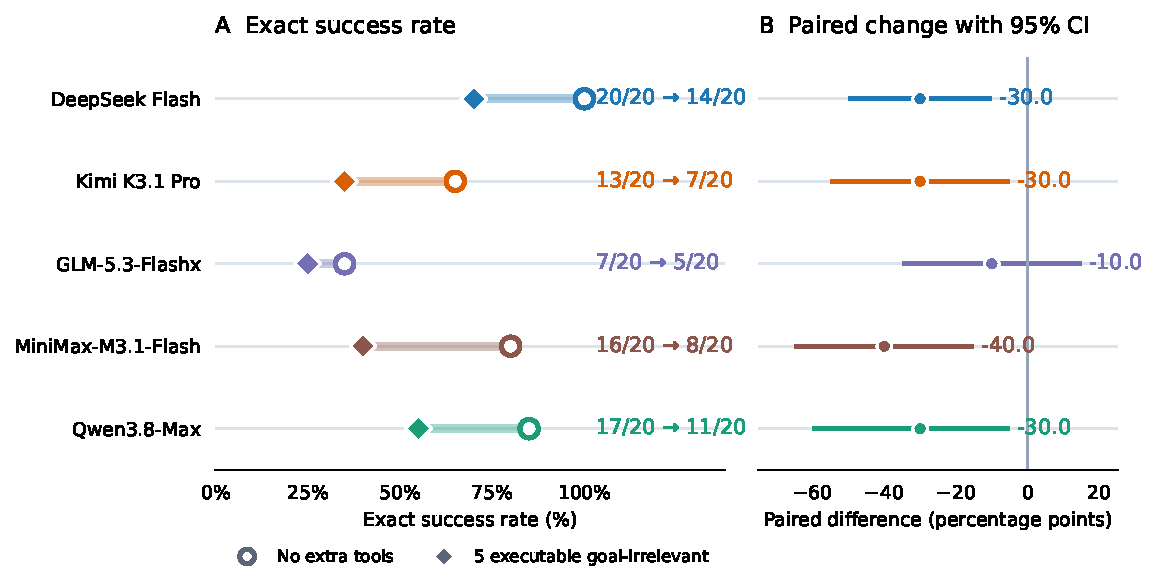
\includegraphics[width=\linewidth]{../figures/figure1_main20_effect.pdf}
\caption{Exact success under zero and five connected-compatible distractors.
Generated from the formal main analysis.}
\label{fig:main}
\end{figure}

\subsection{Dose pattern on shared graphs}
\begin{table}[htbp]
\centering
\caption{Exact success rate for 0, 2, and 5 executable goal-irrelevant tools on 15 shared graphs for five model aliases.}
\label{tab:dose}
\footnotesize
\setlength{\tabcolsep}{3pt}
\renewcommand{\arraystretch}{1.08}
\begin{tabularx}{\textwidth}{>{\raggedright\arraybackslash}Xrrrrr}
\toprule
Model & 0 & 2 & 5 & Delta 2-0 [95\% CI] & Delta 5-0 [95\% CI] \\
\midrule
DeepSeek-V4.1-Flash & 15/15 & 15/15 & 10/15 & +0.0 pp [+0.0, +0.0] & -33.3 pp [-60.0, -13.3] \\
Kimi & 11/15 & 7/15 & 5/15 & -26.7 pp [-46.7, -6.7] & -40.0 pp [-66.7, -20.0] \\
GLM & 4/15 & 2/15 & 3/15 & -13.3 pp [-40.0, +13.3] & -6.7 pp [-33.3, +20.0] \\
MiniMax & 12/15 & 13/15 & 5/15 & +6.7 pp [-20.0, +33.3] & -46.7 pp [-73.3, -20.0] \\
Qwen & 12/15 & 12/15 & 8/15 & +0.0 pp [-26.7, +26.7] & -26.7 pp [-60.0, +6.7] \\
\bottomrule
\end{tabularx}
\par\parbox{\linewidth}{\raggedright\footnotesize Source: \texttt{results/\allowbreak{}funcbench-dose-five-model-20261101/\allowbreak{}}.}
\par\parbox{\linewidth}{\raggedright\footnotesize Cells are correct/trials; deltas are paired proportions in percentage points. These data indicate model-specific plateaus or threshold-like patterns, not a common parametric threshold.}
\end{table}


DeepSeek and Qwen remain flat between zero and two distractors and then decline
at five. Kimi declines at two and again at five. GLM is already low at zero,
declines further at two, and rises by one success at five. A common linear
response or a single stable threshold is not supported. ``Threshold-like'' is a
description of the sufficient-case pattern, not an estimated breakpoint.

\begin{figure}[t]
\centering
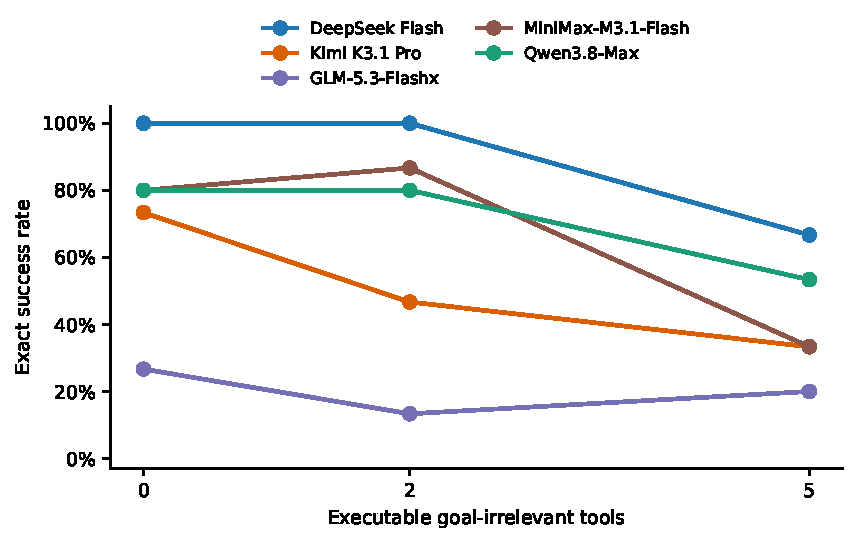
\includegraphics[width=0.82\linewidth]{../figures/figure2_dose_response.pdf}
\caption{Sufficient-case rates for 0, 2, and 5 connected-compatible distractors
on 15 shared graphs for five model aliases.}
\label{fig:dose}
\end{figure}

\subsection{Distractor affordance controls}
\begin{table}[htbp]
\centering
\caption{Tool-usability controls on the same 15 core graphs. All five-extra-tool conditions expose the same number of tools, and all five model aliases are included.}
\label{tab:usability-controls}
\footnotesize
\setlength{\tabcolsep}{3pt}
\renewcommand{\arraystretch}{1.08}
\begin{tabularx}{\textwidth}{>{\raggedright\arraybackslash}Xrrrr}
\toprule
Model & 0 & Disconnected 5 & Connected-incompatible 5 & Executable goal-irrelevant 5 \\
\midrule
DeepSeek & 15/15 (100.0\%) & 14/15 (93.3\%) & 12/15 (80.0\%) & 10/15 (66.7\%) \\
Kimi & 11/15 (73.3\%) & 10/15 (66.7\%) & 7/15 (46.7\%) & 5/15 (33.3\%) \\
GLM & 4/15 (26.7\%) & 8/15 (53.3\%) & 4/15 (26.7\%) & 3/15 (20.0\%) \\
MiniMax & 12/15 (80.0\%) & 13/15 (86.7\%) & 11/15 (73.3\%) & 5/15 (33.3\%) \\
Qwen & 12/15 (80.0\%) & 14/15 (93.3\%) & 8/15 (53.3\%) & 8/15 (53.3\%) \\
\bottomrule
\end{tabularx}
\par\parbox{\linewidth}{\raggedright\footnotesize Source: \texttt{results/\allowbreak{}funcbench-control-five-model-analysis-20261101/\allowbreak{}metric\_summary.csv}.}
\par\parbox{\linewidth}{\raggedright\footnotesize Each model has 15 trials per condition. The disconnected and connected-incompatible controls do not reproduce the degradation observed with executable goal-irrelevant tools. DeepSeek has one technical/budget failure in each connected condition.}
\end{table}


The connected-compatible condition is lowest for DeepSeek, Kimi, GLM, and
MiniMax and ties the connected-incompatible condition for Qwen. Adding five disconnected
tools does not reproduce the same level of failure. This is the strongest
evidence in the present study against the simplest explanation that ``more tools
necessarily means worse success.'' It is not a complete causal proof that type
compatibility alone causes the effect. The controls change graph structure and
callability together, and each condition has 15 graphs.

\begin{figure}[t]
\centering
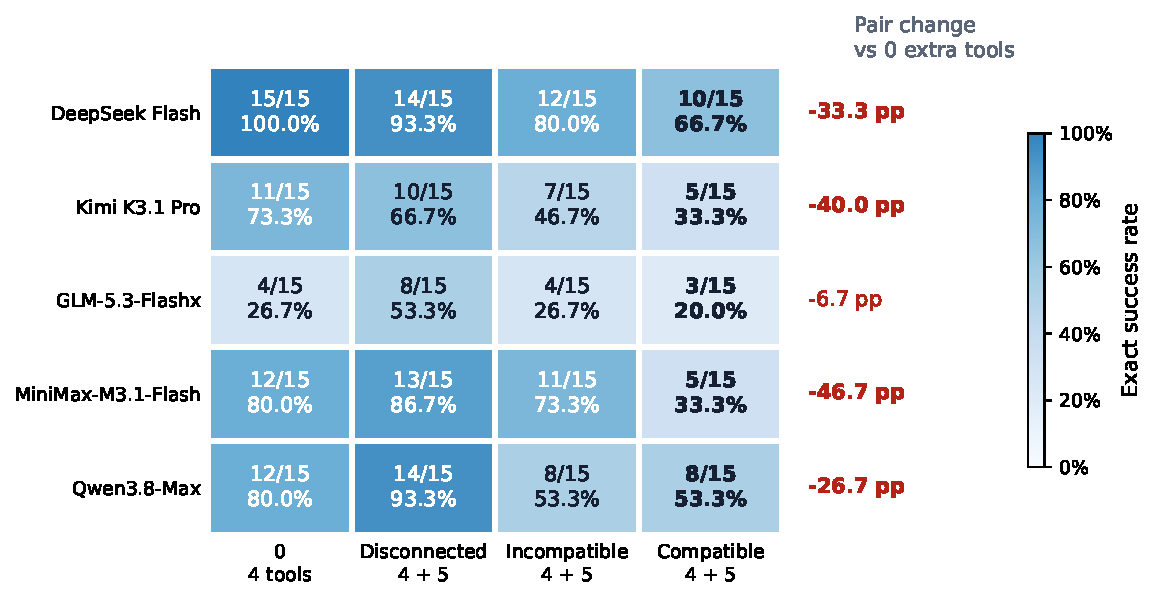
\includegraphics[width=\linewidth]{../figures/figure3_affordance_controls.pdf}
\caption{Tool count is held at five for the three distractor controls for all
five model aliases.}
\label{fig:affordance}
\end{figure}

\subsection{Affordance-Specific Penalty}
\begin{table}[htbp]
\centering
\caption{ASP (historical metric name) reports the average paired loss relative to the same-count disconnected and connected-incompatible controls.}
\label{tab:asp}
\footnotesize
\setlength{\tabcolsep}{3pt}
\renewcommand{\arraystretch}{1.08}
\begin{tabularx}{\textwidth}{>{\raggedright\arraybackslash}Xrrrrrr}
\toprule
Model & D-GI & I-GI & ASP [95\% CI] & Sign-flip p & Holm p & +/0/- graphs \\
\midrule
DeepSeek-V4.1-Flash & +26.7 pp & +13.3 pp & +20.0 pp [-3.3, +43.3] & 0.219 & 0.562 & 5/8/2 \\
Kimi K3.1 Pro & +33.3 pp & +13.3 pp & +23.3 pp [+3.3, +43.3] & 0.094 & 0.375 & 6/8/1 \\
GLM-5.3-Flashx & +33.3 pp & +6.7 pp & +20.0 pp [-6.7, +43.3] & 0.246 & 0.562 & 7/6/2 \\
MiniMax-M3.1-Flash & +53.3 pp & +40.0 pp & +46.7 pp [+23.3, +70.0] & 0.007 & 0.034 & 10/4/1 \\
Qwen3.8-Max & +40.0 pp & +0.0 pp & +20.0 pp [-3.3, +43.3] & 0.188 & 0.562 & 6/7/2 \\
\bottomrule
\end{tabularx}
\par\parbox{\linewidth}{\raggedright\footnotesize Source: \texttt{results/\allowbreak{}funcbench-control-five-model-analysis-20261101/\allowbreak{}asp/\allowbreak{}asp\_summary.csv}.}
\par\parbox{\linewidth}{\raggedright\footnotesize D-GI is the exact success rate under disconnected tools minus that under executable goal-irrelevant tools; I-GI is the corresponding difference for connected-incompatible tools. Intervals resample graphs; p-values use exact two-sided sign flips; Holm adjustment covers five models.}
\end{table}


All five ASP point estimates are positive, ranging from \ASPRangeLowPP{} to
\ASPRangeHighPP{} percentage points. MiniMax has the largest estimate
(\MiniMaxASPP{} points, 95\% CI
[\MiniMaxASPLowPP, \MiniMaxASPHighPP]) and is the only model that remains below
0.05 after Holm correction (\MiniMaxASPHolmP). The other intervals include
zero. The result establishes a consistent direction across five models but not
a statistically homogeneous model property.

\begin{figure}[t]
\centering
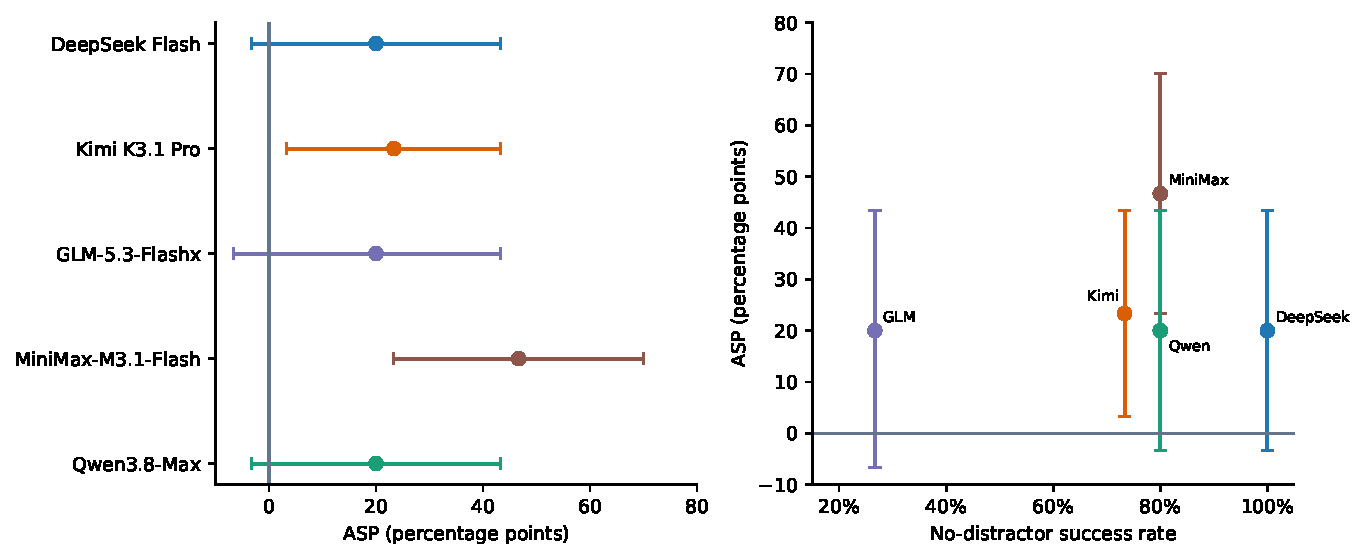
\includegraphics[width=\linewidth]{../figures/figure5_asp_profile.pdf}
\caption{ASP forest intervals and the descriptive relation between baseline
success and ASP.}
\label{fig:asp}
\end{figure}

\subsection{Schema-matched sealed-twin probe}
\begin{table}[htbp]
\centering
\caption{EAP (historical metric name) reports the paired loss between sealed and executable goal-irrelevant tools on 10 shared graphs.}
\label{tab:eap}
\footnotesize
\setlength{\tabcolsep}{3pt}
\renewcommand{\arraystretch}{1.08}
\begin{tabularx}{\textwidth}{>{\raggedright\arraybackslash}Xrrrrrr}
\toprule
Model & Executable & Sealed & EAP [95\% CI] & Sign-flip p & Holm p & +/0/- graphs \\
\midrule
DeepSeek-V4.1-Flash & 7/10 & 9/10 & +20.0 pp [+0.0, +50.0] & 0.500 & 1.000 & 2/8/0 \\
Kimi K3.1 Pro & 4/10 & 4/10 & +0.0 pp [-30.0, +30.0] & 1.000 & 1.000 & 1/8/1 \\
GLM-5.3-Flashx & 1/10 & 5/10 & +40.0 pp [+10.0, +70.0] & 0.125 & 0.625 & 4/6/0 \\
MiniMax-M3.1-Flash & 3/10 & 7/10 & +40.0 pp [+10.0, +70.0] & 0.125 & 0.625 & 4/6/0 \\
Qwen3.8-Max & 6/10 & 8/10 & +20.0 pp [-20.0, +60.0] & 0.625 & 1.000 & 3/6/1 \\
\bottomrule
\end{tabularx}
\par\parbox{\linewidth}{\raggedright\footnotesize Source: \texttt{results/\allowbreak{}funcbench-sealed-probe-analysis-20261101/\allowbreak{}eap/\allowbreak{}eap\_summary.csv}.}
\par\parbox{\linewidth}{\raggedright\footnotesize Executable and sealed tools have identical names, descriptions, schemas, order, prompts, required graphs, and target values. Only runtime execution differs. Positive EAP means that sealing improved the exact success rate.}
\end{table}


EAP is +20.0 points for DeepSeek, 0.0 for Kimi, +40.0 for GLM, +40.0 for
MiniMax, and +20.0 for Qwen. GLM and MiniMax have bootstrap intervals excluding
zero, but no model survives Holm correction. This is exploratory evidence that
actual executability contributes to failure, not a completed causal mechanism.

\begin{figure}[t]
\centering
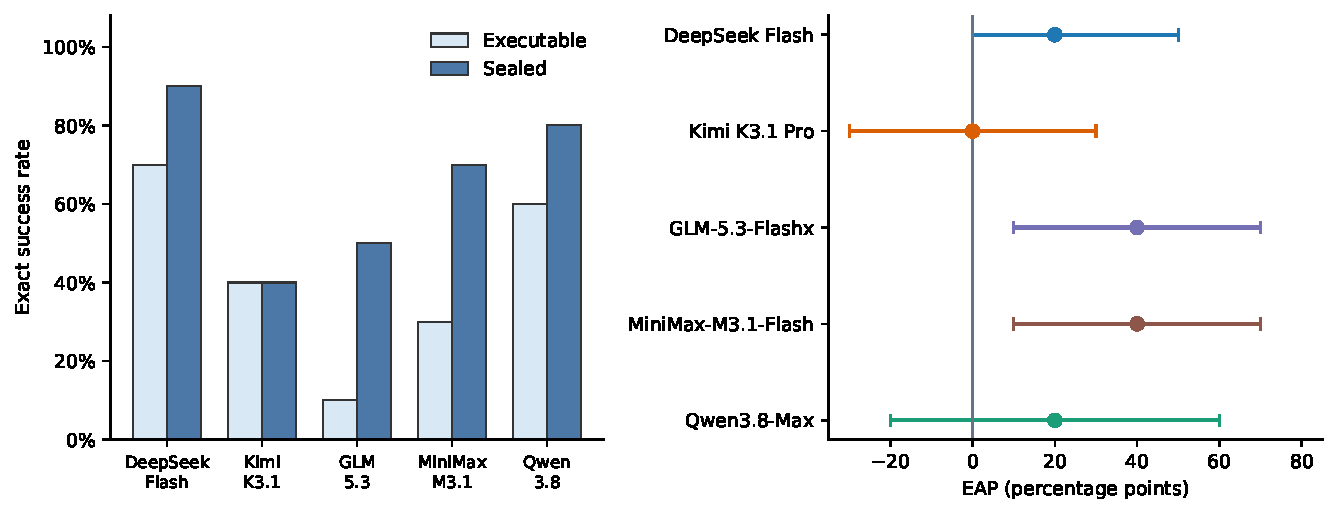
\includegraphics[width=\linewidth]{../figures/figure7_sealed_probe.pdf}
\caption{Schema-matched executable and sealed tools on 10 shared graphs.}
\label{fig:sealed}
\end{figure}

\subsection{Trace diagnostics and error distribution}
Across the 200 main trials there are 118 correct outcomes, 23 wrong argument
values, 29 premature dependency uses, 22 irrelevant function calls, seven
premature final answers, and one technical/budget failure. At zero distractors,
73 trials are correct, 14 have wrong arguments, and 13 use a dependency
prematurely. At five distractors, 45 are correct, nine have wrong arguments, 16
use a dependency prematurely, 22 call an irrelevant function, seven end
prematurely, and one is technical.

\begin{table}[htbp]
\centering
\caption{Structured tool-trace diagnostics for five model aliases on the 20-graph main experiment.}
\label{tab:trace}
\footnotesize
\setlength{\tabcolsep}{3pt}
\renewcommand{\arraystretch}{1.08}
\begin{tabularx}{\textwidth}{>{\raggedright\arraybackslash}Xrrrrrr}
\toprule
Model & Extra tools & Req. & Sel. & Order & Arg. & Fidelity \\
\midrule
DeepSeek-V4.1-Flash & 0 & 1.000 & 1.000 & 1.000 & 1.000 & 1.000 \\
DeepSeek-V4.1-Flash & 5 & 0.938 & 0.750 & 0.970 & 0.883 & 0.885 \\
Kimi & 0 & 1.000 & 1.000 & 1.000 & 0.850 & 0.963 \\
Kimi & 5 & 0.938 & 0.660 & 1.000 & 0.839 & 0.859 \\
GLM & 0 & 1.000 & 1.000 & 1.000 & 0.800 & 0.950 \\
GLM & 5 & 0.762 & 0.578 & 1.000 & 0.828 & 0.792 \\
MiniMax & 0 & 1.000 & 1.000 & 1.000 & 0.903 & 0.976 \\
MiniMax & 5 & 0.938 & 0.628 & 0.988 & 0.888 & 0.860 \\
Qwen & 0 & 1.000 & 1.000 & 1.000 & 0.925 & 0.981 \\
Qwen & 5 & 0.900 & 0.693 & 0.988 & 0.975 & 0.889 \\
\bottomrule
\end{tabularx}
\par\parbox{\linewidth}{\raggedright\footnotesize Source: \texttt{results/\allowbreak{}funcbench-main20-five-model-analysis-20261101/\allowbreak{}metric\_summary.csv}.}
\par\parbox{\linewidth}{\raggedright\footnotesize Trace fidelity is the equal-weight mean of required recall, selection precision, dependency order, and argument score; it is diagnostic, not a replacement for exact success.}
\end{table}


Selection precision drops for every model when distractors are present.
Required recall drops for DeepSeek, Kimi, and GLM and remains high for Qwen.
Dependency order remains at or near one. Argument scores are not uniformly worse:
Kimi is slightly lower under distractors, while Qwen and GLM are slightly higher
in this aggregate, with GLM still starting from a low baseline.

A supplementary stricter check found no main trial that was wrong despite an
exact required-function set, dependency-order score 1, and argument score 1.
This does not establish mediation. It does show that the observed end-to-end
decline is concentrated in trajectories where at least one structural component
fails.

\begin{figure}[t]
\centering
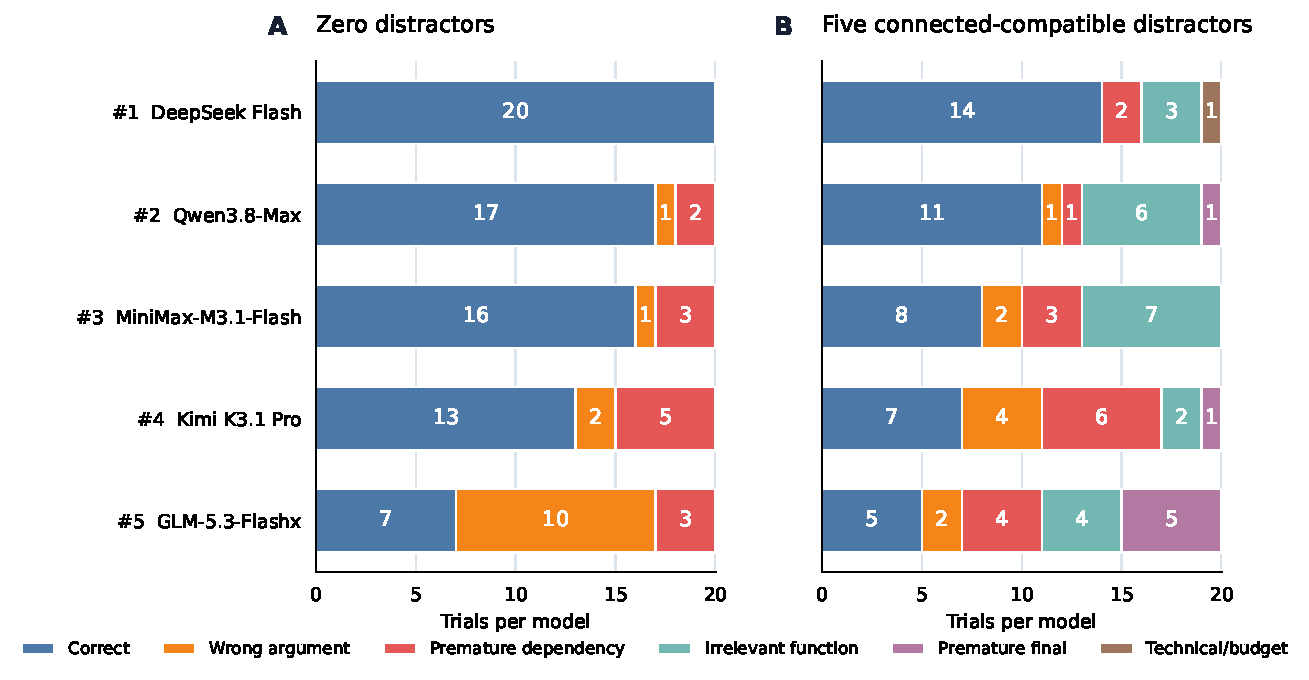
\includegraphics[width=\linewidth]{../figures/figure4_error_taxonomy.pdf}
\caption{Primary error categories by condition for the five model aliases.}
\label{fig:errors}
\end{figure}

\section{Interventions}

\paragraph{State reminder.}
We repeat already produced variable values in the prompt while keeping the same
core graph and connected-compatible distraction. On four paired graphs, success
is 3/4 to 3/4 for DeepSeek, 3/4 to 2/4 for Kimi, 1/4 to 1/4 for GLM, 2/4 to
2/4 for MiniMax, and 3/4 to 3/4 for Qwen. There is no net increase. Kimi moves one graph from correct to
incorrect. One GLM graph and one Kimi graph show opposite-direction transitions;
these are too few observations to interpret as a stable benefit.

\paragraph{Prerequisite hiding.}
The second intervention hides tools whose input dependencies have not yet been
produced. On eight graph-matched connected-compatible instances, success falls
from 5/8 to 1/8 for DeepSeek, 3/8 to 2/8 for Kimi, 1/8 to 0/8 for GLM, 3/8 to
1/8 for MiniMax, and 4/8 to 1/8 for Qwen. The paired deltas are $-50$, $-12.5$,
$-12.5$, $-25.0$, and $-37.5$ percentage points.

\begin{table}[htbp]
\centering
\caption{Two same-graph interventions for five model aliases: prerequisite hiding on eight graphs and a state reminder on four graphs.}
\label{tab:interventions}
\footnotesize
\setlength{\tabcolsep}{3pt}
\renewcommand{\arraystretch}{1.08}
\begin{tabularx}{\textwidth}{>{\raggedright\arraybackslash}Xr>{\raggedright\arraybackslash}X>{\raggedright\arraybackslash}X>{\raggedright\arraybackslash}X}
\toprule
Model & Prerequisite hiding: unhidden -> hidden & Hiding delta & Reminder: baseline -> treated & W->R / R->W \\
\midrule
DeepSeek-V4.1-Flash & 5/8 -> 1/8 & -50.0 pp & 3/4 -> 3/4 & 0 / 0 \\
Kimi K3.1 Pro & 3/8 -> 2/8 & -12.5 pp & 3/4 -> 2/4 & 0 / 1 \\
GLM-5.3-Flashx & 1/8 -> 0/8 & -12.5 pp & 1/4 -> 1/4 & 1 / 1 \\
MiniMax-M3.1-Flash & 3/8 -> 1/8 & -25.0 pp & 2/4 -> 2/4 & 0 / 0 \\
Qwen3.8-Max & 4/8 -> 1/8 & -37.5 pp & 3/4 -> 3/4 & 0 / 0 \\
\bottomrule
\end{tabularx}
\par\parbox{\linewidth}{\raggedright\footnotesize Source: \texttt{results/\allowbreak{}funcbench-gating-five-model-analysis-20261101/\allowbreak{}intervention/\allowbreak{}intervention\_effect\_summary.csv and results/\allowbreak{}funcbench-reminder-five-model-analysis-20261101/\allowbreak{}trial\_failures.csv}.}
\par\parbox{\linewidth}{\raggedright\footnotesize W->R denotes wrong-to-right and R->W denotes right-to-wrong. Neither intervention yields a positive net repair.}
\end{table}


The gating result is not just ``no improvement'': every model declines. A
descriptive transition analysis shows that previously correct DeepSeek and Qwen
trials become irrelevant-function or premature-final failures after gating. The
changed candidate set may alter the model's plan rather than merely remove an
invalid action. We therefore do not recommend tool hiding as a general repair.

\section{Discussion}

\paragraph{Tool count is an insufficient task-description variable.}
In this study, five disconnected tools do not reproduce the degradation observed
for five connected-compatible tools on the same eight graphs. The relevant data
property is therefore likely closer to \emph{executable, goal-irrelevant
affordance} than to candidate count alone. This distinction matters when
constructing a benchmark: two nine-tool tasks can pose different selection and
state-tracking problems depending on whether the extra branches can run. The
controls support a hypothesis, not a complete causal model. More graph seeds and
finer intermediate controls are needed to separate connectedness, type
compatibility, and executability.

\paragraph{Failure is selection and state execution, not only parsing.}
All five models lose function-selection precision under connected-compatible
distractors. The error taxonomy includes wrong arguments, premature dependency
use, irrelevant calls, and premature final answers. This is consistent with the
view that multi-step tool use requires persistent goal state while multiple
valid actions are available. The trace scores are descriptive evidence for that
interpretation; they are not an identified causal pathway.

\paragraph{Negative interventions are useful benchmark evidence.}
The reminder and gating experiments test two plausible state-support strategies.
Neither improves exact success. A paper that reported only aggregate degradation
could suggest that exposing fewer tools or repeating state should help. These
graph-matched negative results challenge that assumption and motivate
interventions that preserve the candidate set while validating argument
provenance or goal consistency.

\section{Limitations}

The main effect has 20 graph clusters, while affordance controls and gating have
eight and the reminder has four. All main results are at dependency depth three.
The main cells use one temperature-1 generation, so repeated-sampling variance is
not yet estimated. The study uses five API aliases from one function-dependency
family. Every analysis panel includes all five models. Provider aliases may
change behind an endpoint; dates and configurations
are recorded, but immutable provider snapshots are unavailable. Automated
primary error labels and trace metrics have not been independently double-coded.
The control conditions vary connectedness, type compatibility, and executable
affordance together. The 15-graph dose pattern is descriptive and does not
support a stable complexity threshold. ASP and EAP are derived contrasts, and
the 10-graph sealed probe is underpowered for a definitive mechanism claim.
Finally, code, generated graph data,
license, hosting, and maintenance require finalization.

\impact{This work evaluates API-served models using synthetically generated
function graphs and does not involve human subjects or user data. A public
release should avoid exposing provider credentials or raw account metadata. If
generated tools are later connected to real APIs, benchmark examples should
remain isolated from production systems and should not encourage unsafe
autonomous action. The positive impact is improved evaluation practice:
benchmark builders can report whether irrelevant tools are merely present or
actually executable, and can audit the required task independently of the
distractor layer. A negative impact is overinterpretation. A high score on this
narrow suite cannot certify safe or reliable agents, and a low score cannot
establish general model quality. We therefore report condition-specific
evidence and negative interventions rather than a leaderboard.}

\acks{Author names, affiliations, funding, competing interests, and
acknowledgements remain to be completed. No funding disclosure is asserted in
this working draft.}

\bibliography{references}

\appendix
\section{Valid-Run Sensitivity and Additional Trace Checks}

The main analysis retains the single technical failure. Excluding it does not
change the direction: DeepSeek's distractor success becomes 14/19.

\begin{table}[htbp]
\centering
\caption{Sensitivity to technical/budget failures and end-to-end trace completeness.}
\label{tab:validtrace}
\footnotesize
\setlength{\tabcolsep}{3pt}
\renewcommand{\arraystretch}{1.08}
\begin{tabularx}{\textwidth}{>{\raggedright\arraybackslash}Xrrrrrr}
\toprule
Model & Extra tools & Attempts & Technical/budget failures & Success among valid runs & Complete structural trace & Wrong despite complete trace \\
\midrule
DeepSeek-V4.1-Flash & 0 & 20 & 0 & 20/20 & 20/20 & 0 \\
DeepSeek-V4.1-Flash & 5 & 20 & 1 & 14/19 & 10/20 & 0 \\
Kimi & 0 & 20 & 0 & 13/20 & 13/20 & 0 \\
Kimi & 5 & 20 & 0 & 7/20 & 4/20 & 0 \\
GLM & 0 & 20 & 0 & 7/20 & 7/20 & 0 \\
GLM & 5 & 20 & 0 & 5/20 & 2/20 & 0 \\
MiniMax & 0 & 20 & 0 & 16/20 & 16/20 & 0 \\
MiniMax & 5 & 20 & 0 & 8/20 & 3/20 & 0 \\
Qwen & 0 & 20 & 0 & 17/20 & 17/20 & 0 \\
Qwen & 5 & 20 & 0 & 11/20 & 7/20 & 0 \\
\bottomrule
\end{tabularx}
\par\parbox{\linewidth}{\raggedright\footnotesize Source: \texttt{results/\allowbreak{}funcbench-main20-five-model-analysis-20261101/\allowbreak{}trial\_failures.csv}.}
\par\parbox{\linewidth}{\raggedright\footnotesize A complete structural trace requires the exact required-function set, dependency order score 1, and argument score 1. The table is supplementary because final-answer correctness remains the primary outcome.}
\end{table}


The generated supplement also contains graph-matched gating error transitions.
Those transitions are exploratory because each model has eight pairs and the
primary categories are automated.

\section{Reproducibility and Artifact Plan}

The formal run configurations, analysis summaries, graph fingerprints, and
derived paper tables are retained in the project. A release should include
deterministic graph generation code, exact prompts and tool schemas, analysis
code, model configuration snapshots, sanitized traces, and scripts that
regenerate every table and figure.

Before submission, the following must be supplied: a stable artifact repository
and archival DOI; a release version and license; a public generated-dataset URL
or explicit reviewer-access mechanism; dataset documentation and intended-use
boundaries; hosting and maintenance responsibility; a reproducibility
checklist; and author and conflict-of-interest information.

\end{document}

